% ||||||||||||||||||||||||||||||||||||||||||||||
% Capitulo de Metodologia
% ||||||||||||||||||||||||||||||||||||||||||||||

\chapter{Metodologia}

O presente capítulo descreve todas as etapas do desenvolvimento do projeto, indo desde a configuração do simulador de falhas MFS 
\textsuperscript \textregistered, da empresa SpectraQuest \textsuperscript \textregistered, até a implementação em campo. A metodologia do
desenvolvimento se encontra na figura \ref{fig:metodologia}, onde as etapas estão descritas em forma de fluxo de trabalho.

\begin{figure}[H]
    \caption{Metodologia do Projeto}
    \begin{center}
        \includegraphics[scale=1.1, page=3]{metodologia/img/software.pdf}
    \end{center}
    \fonte{Elaborado pelo autor.} 
    \label{fig:metodologia}
\end{figure}

Dentre as etapas descritas na imagem anterior, a simulação, desenvolvimento do software, integração de SH (Software e Hardware) e implementação
estão descritas com detalhes nos subcapítulos a seguir.


%++++++++++++++++++++++++++++++++++++++++++++++++++++++++++++++++
% 
%++++++++++++++++++++++++++++++++++++++++++++++++++++++++++++++++

\section{Configurações das Simulações}

Como dito anteriormente no fluxo de desenvolvimento, fez se o uso de simulações antes da implementação do sistema.
Para isso, fui utilizado um simulador de falhas em motores elétricos de indução e sistemas mancalizados, denominado
MFS \textsuperscript \textregistered (\textit{Machinery Fault Simulator} - simulador de falhas em máquinas), que pode ser visto na figura 
\ref{fig:real_plant}. O simulador é composto por um motor elétrico de indução trifásico de 1 HP, o qual está conectado com um eixo via um 
acoplamento. Esse eixo possui dois discos dourados furado, onde é possível se colocar cargas para criar um desbalanceamento no sistema.

\begin{figure}[H]
    \caption{Estrutura do simulador MFS \textsuperscript \textregistered.}
    \begin{center}
        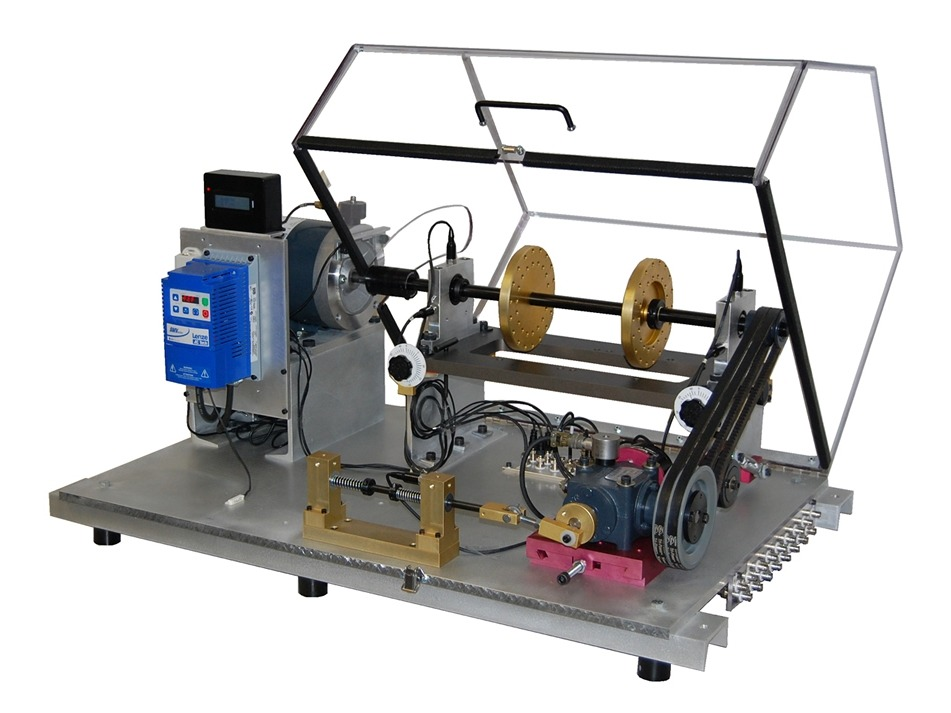
\includegraphics[scale=.4]{metodologia/img/real_plant.jpeg}
    \end{center}
    \fonte{\citeonline{SpectraQuest2011}.} 
    \label{fig:real_plant}
\end{figure}

Para a realização dos testes, diversas combinações de falhas, frequências do inversor de frequências e frequências de amostragem foram
utilizadas, para se entender as dinâmicas das falhas diferentes condições de testes. A planta possui diversos acelerômetros e um sensor
de corrente, que está amostra uma das fases da alimentação. As falhas que foram inseridas nos testes foram a de desalinhamento dos
mancais e o desbalanceamento das cargas. Essas partes podem ser vistas na figura \ref{fig:lateral_desenho}.

\begin{figure}[H]
    \caption{Desenho simplificado da Planta.}
    \begin{center}
        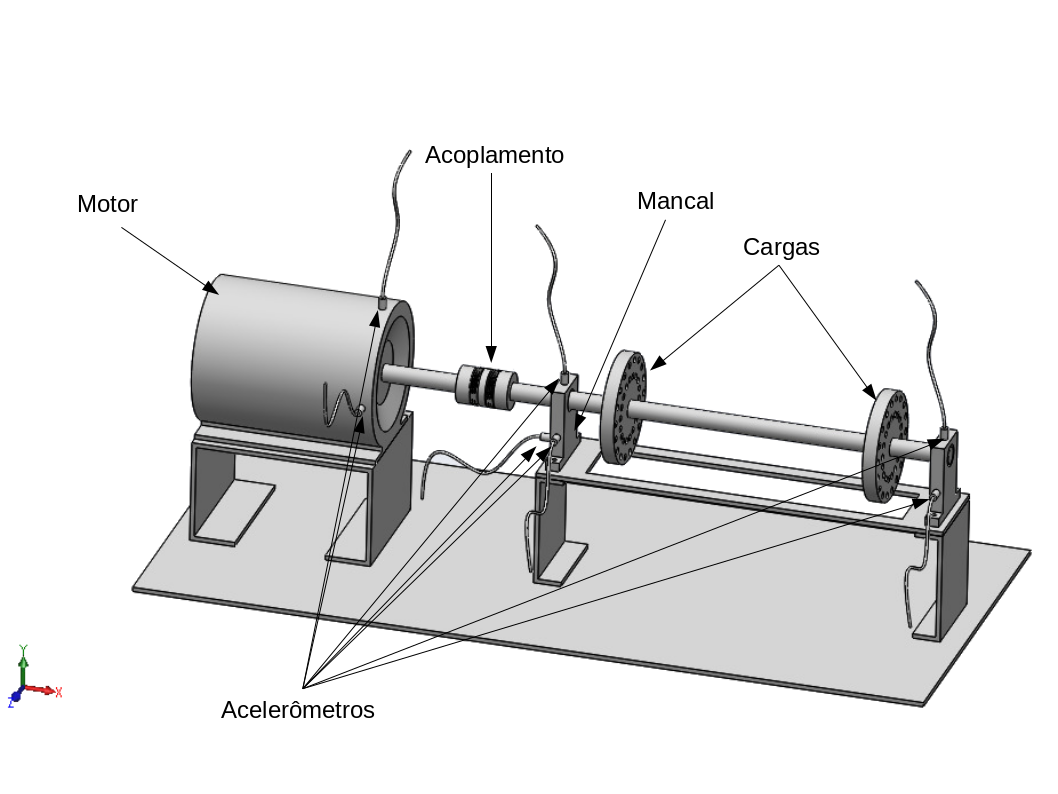
\includegraphics[scale=.5]{metodologia/img/lateral_desenho.png}
    \end{center}
    \fonte{Elaborado pelo Autor.} 
    \label{fig:lateral_desenho}
\end{figure}

A tabela \ref{tab:simulador} contem as combinações de testes que foram realizados. Onde DA é desalinhamento e DB é desbalanceamento.
Cada um destes arquivos gerados possuem 9 colunas de dados, que correspondem aos 7 acelerômetros, 1 tacógrafo e um transformador de
corrente.

\begin{table}[H]
    \caption{Testes realizados.}
    \label{tab:simulador}
    \centering%
    \begin{minipage}{\textwidth}
      \begin{tabular*}{\textwidth}{cccc}
        \hline
        {Nome}                   & Falha                     & Freq. do motor [Hz] & Amostragem [kHz]\\ \hline
        \hline
        Bom                      &  Sem                      &      60             &    25  \\ 
        Misa15                   &  DA de 15 mils            &      60             &    10  \\
        Misa35\_10k\_20Hz        &  DA de 35 mils            &      20             &    25  \\
        Misa35\_10k\_20Hz\_unb   &  DA de 35 mils e DB       &      20             &    25  \\
        Misa35\_10k\_30Hz\_unb   &  DA de 35 mils e DB       &      30             &    25  \\
        Misa35\_10k\_40Hz        &  DA de 35 mils            &      40             &    25  \\
        Misa35\_10k\_5Hz         &  DA de 35 mils            &      5              &    25  \\
        Misa35\_10k\_80Hz        &  DA de 35 mils            &      80             &    25  \\
        Misa35\_8k               &  DA de 35 mils            &      20             &    20  \\ \hline
      \end{tabular*}
      \fonte{Elaborado pelo Autor.} 
    \end{minipage}
  \end{table}
  
Após a apresentação de como foram realizados os testes no simulador, é possível aplicar as topologias propostas no presente trabalho nos
dados gerados. Após a etapa de simulação e análise dos dados, com os resultados obtidos, foi possível o início do desenvolvimento do software,
que será descrito na próxima etapa. 


%++++++++++++++++++++++++++++++++++++++++++++++++++++++++++++++++
% 
%++++++++++++++++++++++++++++++++++++++++++++++++++++++++++++++++

\section{Desenvolvimento do Software}

Com a escrita dos requisitos, simulações e análise dos dados das simulações, foi possível o início da etapa de desenvolvimento de software,
que agrega várias ferramentas para entregar um sistema de tempo real para o monitoramento da saúde de motor elétricos de indução. A 
implementação foi dividida em três principais tarefas: Aquisição dos dados, Machine Learning e o monitoramento. A duas primeiras estão
descritas na imagem a seguir.

\begin{figure}[H]
    \caption{Tarefas de Aquisição e Machine Learning}
    \begin{center}
        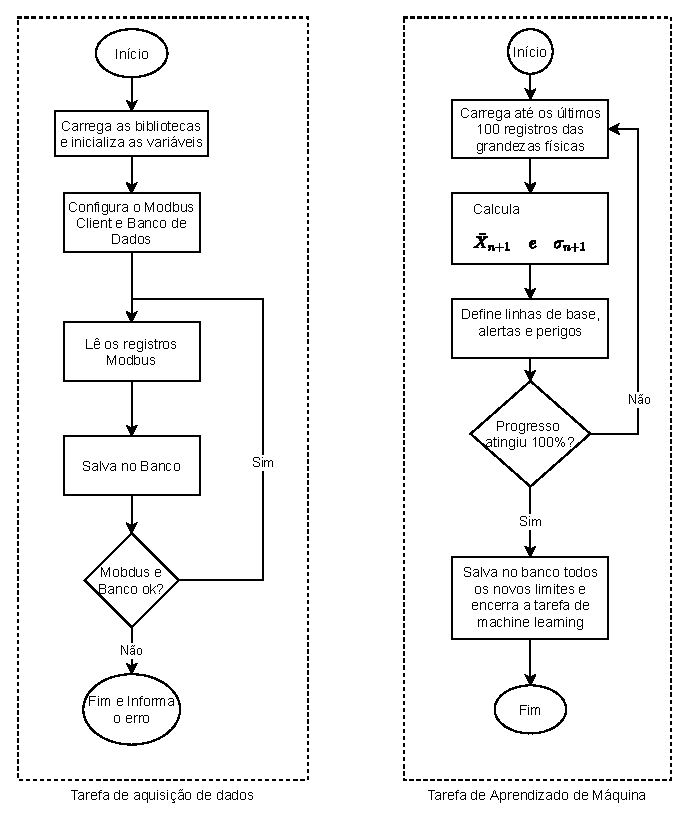
\includegraphics[scale=1, page=1]{metodologia/img/software.pdf}
    \end{center}
    \fonte{Elaborado pelo autor.} 
    \label{fig:tarefa_aq_ml}
\end{figure}

Como podemos ver ******************** falar detalhes do ML
gancho do monitoramento *******************************

\begin{figure}[H]
    \caption{Tarefa de monitoramento}
    \begin{center}
        \includegraphics[scale=1, page=2]{metodologia/img/software.pdf}
    \end{center}
    \fonte{Elaborado pelo autor.} 
    \label{fig:k-means}
\end{figure}


alguns detalhes do monitoramento *********************************
gancho das telas *******************************


\begin{figure}[H]
    \caption{Fluxo de acesso do Software.}
    \begin{center}
        \includegraphics[scale=0.25, page=2]{metodologia/img/fluxo_layout.pdf}
    \end{center}
    \fonte{Elaborado pelo autor.} 
    \label{fig:sensor_exaustor}
\end{figure}

Como podemos ver ******************** falar detalhes do dashboard
gancho pro prox subchapter *******************************

%++++++++++++++++++++++++++++++++++++++++++++++++++++++++++++++++
% 
%++++++++++++++++++++++++++++++++++++++++++++++++++++++++++++++++

\section{Integração entre Software e Hardware}


\begin{table}[H]
    \caption{Especificações do Sensor QM30VT2}
    \label{tab:simulador}
    \centering%
    \begin{minipage}{.45\textwidth}
      \begin{tabular*}{\textwidth}{c|c}
        \hline
        Especificação            & Valores                                     \\ \hline
        \hline
        intervalo de medição     &  0 a $\SI{46}{\milli\metre\per\second}$     \\
        Largura de banda         &  10 a $\SI{4}{\kilo\hertz}$                 \\ 
        Acurácia                 &  $\mp 10 \%$ a $\SI{25}{\celsius}$          \\
        Amostragem               &  $\SI{20}{\kilo\hertz}$                     \\
        Tempo de Amostragem      &  $\SI{0.4}{\second}$                        \\
        Grau de Certificação     &  IP67                                       \\
      \end{tabular*}
      \fonte{Elaborado pelo Autor.} 
    \end{minipage}
  \end{table}



\begin{figure}[H]
    \caption{Diagrama de integração entre sensores e Software.}
    \begin{center}
        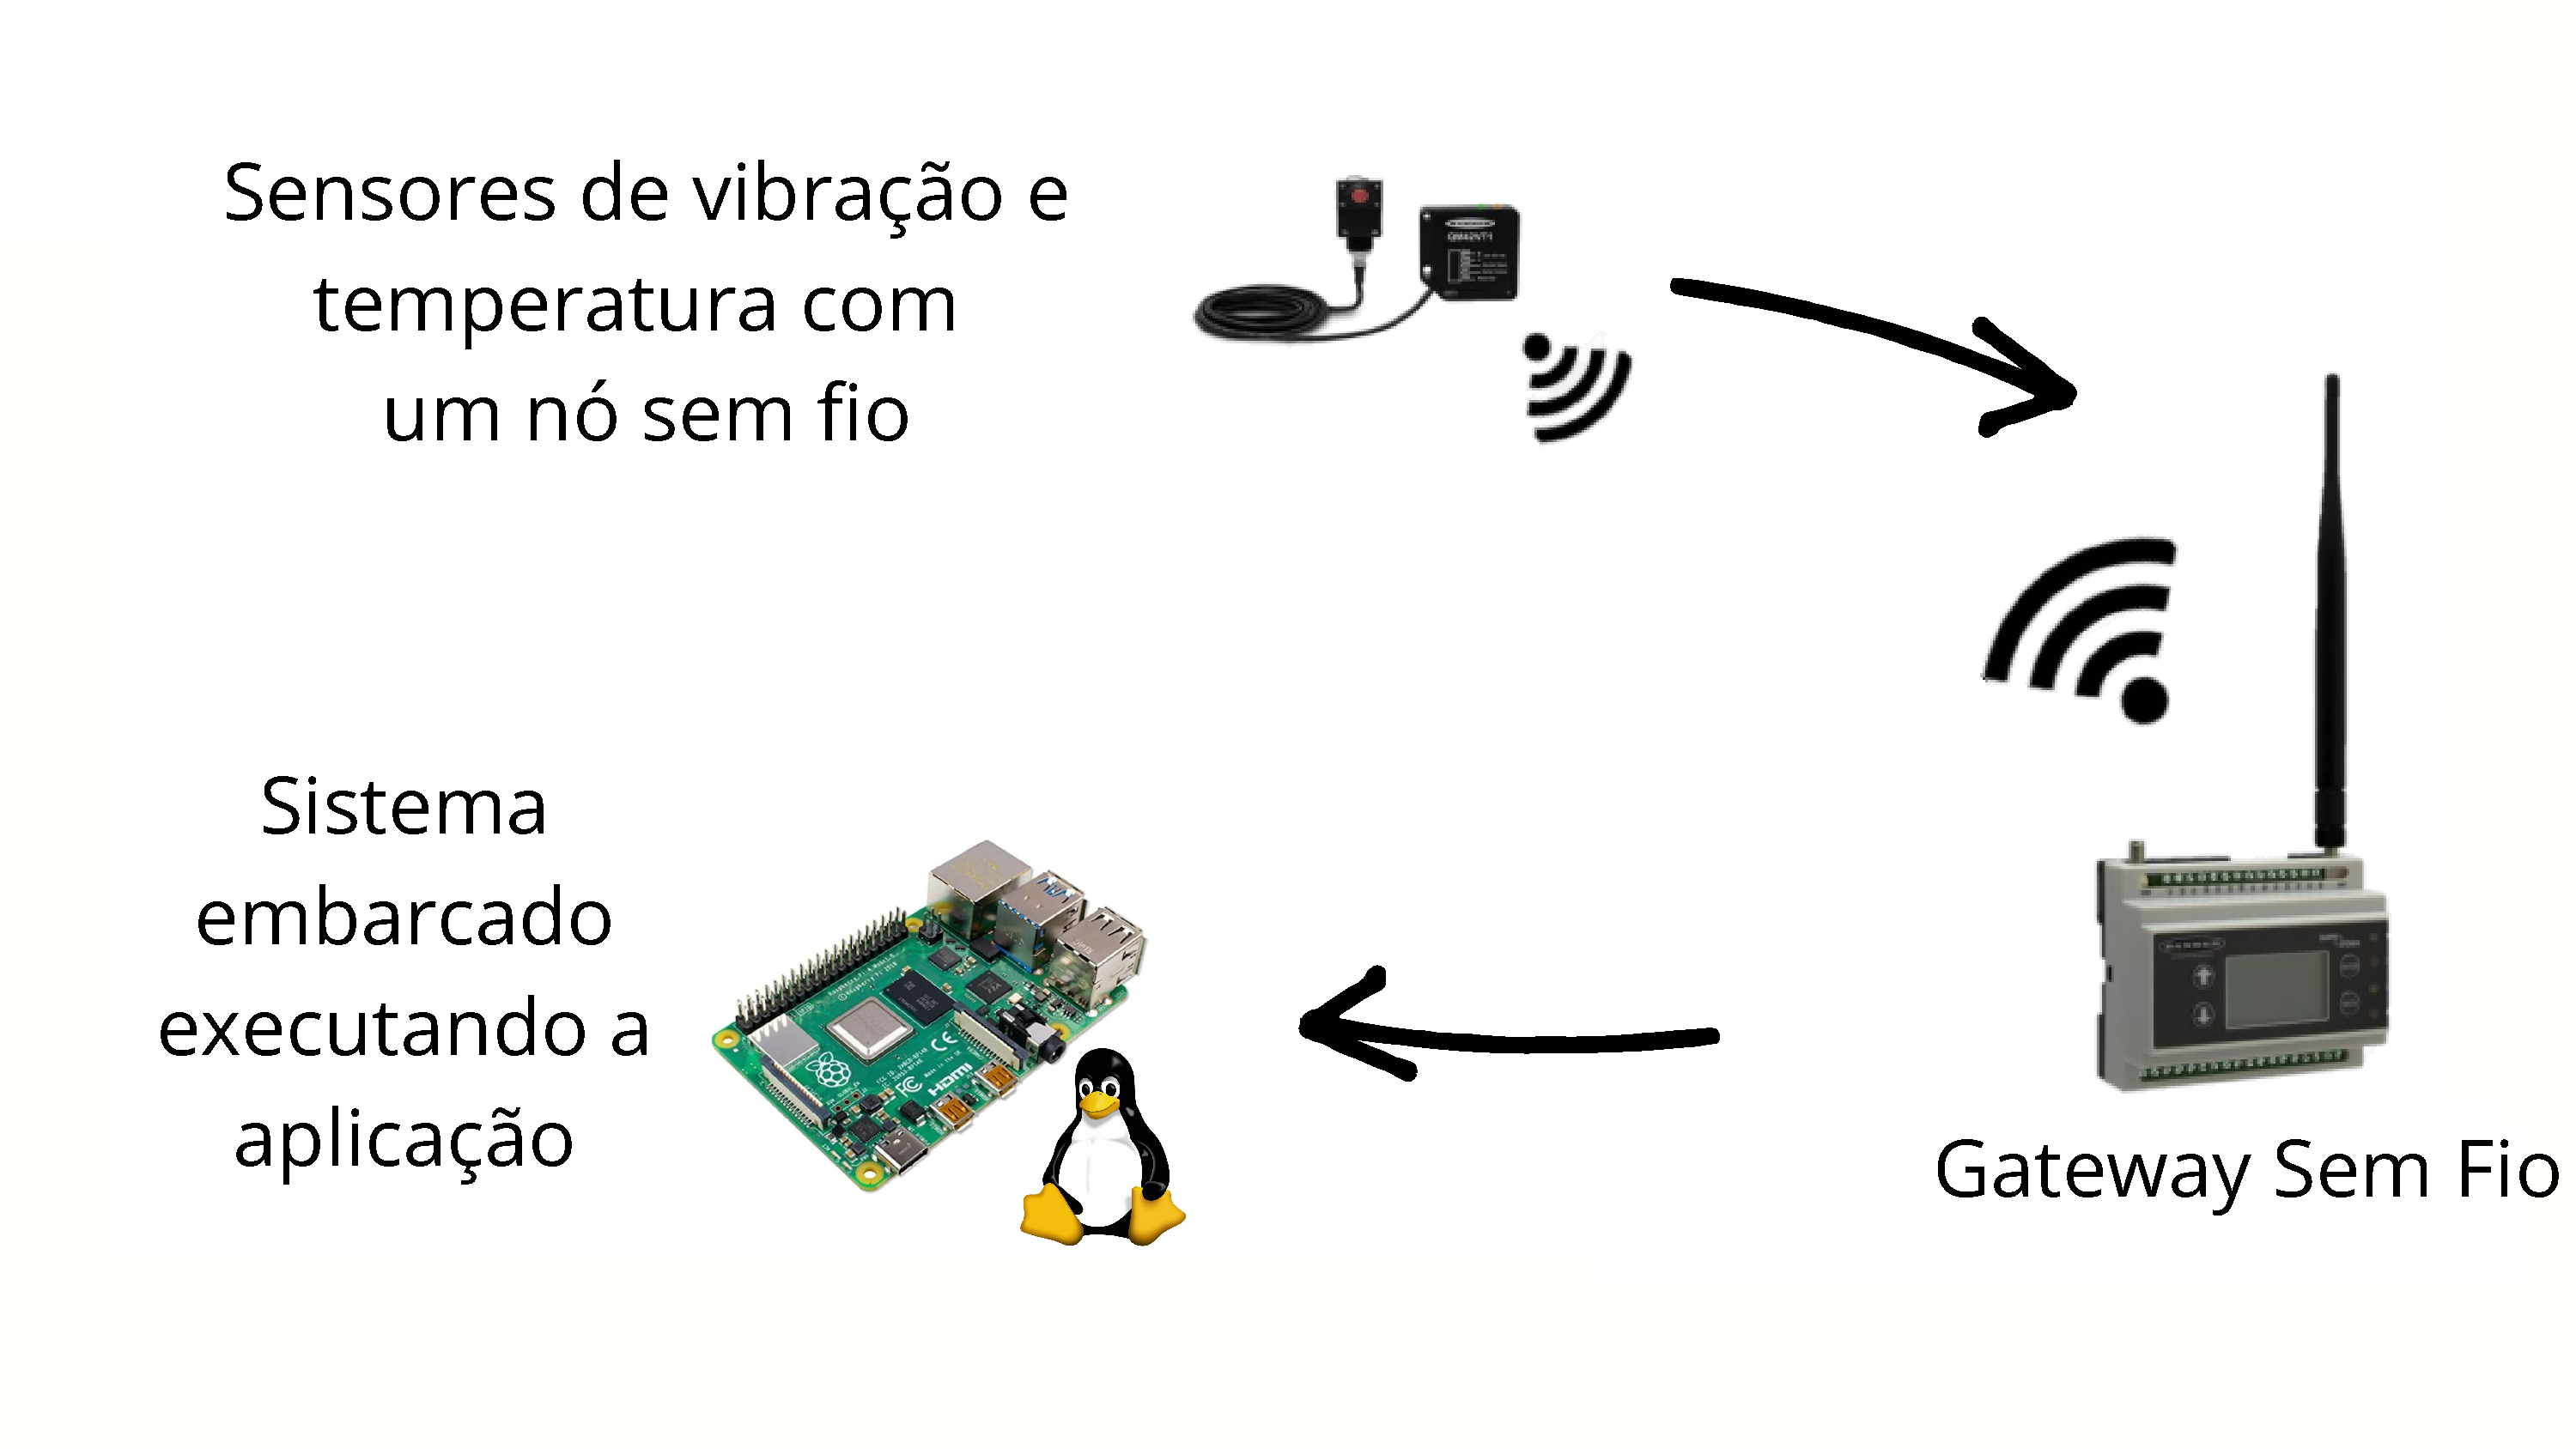
\includegraphics[scale=0.25, page=1]{metodologia/img/fluxo_layout.pdf}
    \end{center}
    \fonte{Adaptado pelo autor.} 
    \label{fig:sensor_exaustor}
\end{figure}


%++++++++++++++++++++++++++++++++++++++++++++++++++++++++++++++++
% 
%++++++++++++++++++++++++++++++++++++++++++++++++++++++++++++++++

\section{Configurações e Implementação em Campo}

Além do ambiente controlado, os conceitos foram aplicados em equipamentos reais e funcionais, que operam 24 horas por dia, 7 dias por semana. 
No decorrer do trabalho, foi possível aplicar em mais de 2 empresas a aplicação. A figura \ref{fig:exautor} representa um exaustor industrial,
um dispositivo que apresenta severas falhas em decorrência do acumulo de partículas que estão no ar. Uma falha num dispositivo desses, acarreta
em uma parada de produção, impactando diretamente no financeiro da empresa.

\begin{figure}[H]
    \caption{Fotografia externa de um exaustor industrical.}
    \begin{center}
        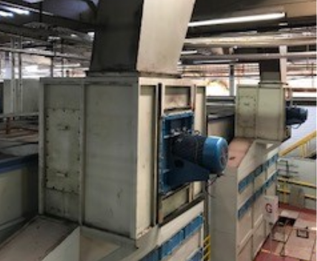
\includegraphics[scale=1.25]{metodologia/img/exaustor.png}
    \end{center}
    \fonte{Forncecida pela empresa.} 
    \label{fig:exautor}
\end{figure}

Em um deste dispositivo foi instalado um sensor industrial de vibração e temperatura, com o objetivo de coletar, processar e armazenar esses
dados, criando um dashboard com o estado de saúde deste motor. A figura \ref{fig:sensor_exaustor} apresenta o sensor instalado.

\begin{figure}[H]
    \caption{Fotografia externa do sensor instalado em um exaustor industrical.}
    \begin{center}
        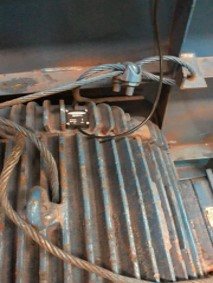
\includegraphics[scale=1.1]{metodologia/img/sensor_exaustor.jpg}
    \end{center}
    \fonte{Forncecida pela empresa.} 
    \label{fig:sensor_exaustor}
\end{figure}



%----------------------------------------------------------------
%  
%----------------------------------------------------------------

% \subsection{K-Means}

% Seguindo a mesma linha da técnica anterior, a técnica K-means foi utilizada com o objetivo de clusterizar os dados em grupos de 4 
% (K=4), pois existem dados de motor bom, com desalinhamento de 15 mils, 35 mils e desbalanceamento. A figura \ref{fig:k-means} apresenta
% a topologia da implementação.


% \begin{figure}[H]
%     \caption{Fluxograma da técnica utilizando K-means.}
%     \begin{center}
%         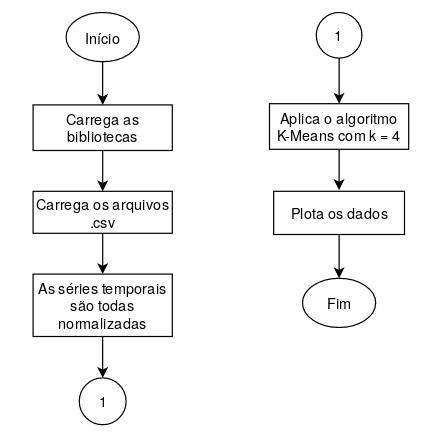
\includegraphics[scale=.65]{metodologia/img/k-means.png}
%     \end{center}
%     \fonte{Elaborado pelo autor.} 
%     \label{fig:k-means}
% \end{figure}

% Já na implementação dessa técnica, foi utilizada a linguagem de programação R, muito difundida dentro da área de aprendizado de máquina.
% O algoritmo também foi executado em uma máquina Linux e de forma offline.


%----------------------------------------------------------------
%  
%----------------------------------------------------------------